\documentclass[times, utf8, diplomski, numeric]{fer}
\usepackage{booktabs}
\usepackage{amsmath}
\usepackage{amssymb}
\usepackage{bm}
\usepackage{algorithm}
\usepackage{algorithmic}
\usepackage{verbatim}
\usepackage{tikz,times}

\usetikzlibrary{arrows}

\tikzset{
  treenode/.style = {align=center, inner sep=0pt, text centered,
    font=\sffamily},
  arn_n/.style = {treenode, circle, white, font=\sffamily\bfseries, draw=black,
    fill=black, text width=1.5em},% arbre rouge noir, noeud noir
  arn_r/.style = {treenode, circle, red, draw=red, 
    text width=1.5em, very thick},% arbre rouge noir, noeud rouge
  arn_x/.style = {treenode, rectangle, draw=black,
    minimum width=0.5em, minimum height=0.5em}% arbre rouge noir, nil
}

\begin{document}
\thesisnumber{1136}
\title{Preporučiteljski sustavi u sveprisutnom računarstvu}
\author{Branimir Pervan}
\maketitle

% Ispis stranice s napomenom o umetanju izvornika rada. Uklonite naredbu
% \izvornik ako želite izbaciti tu stranicu.
\izvornik

% Dodavanje zahvale ili prazne stranice. Ako ne želite dodati zahvalu, naredbu
% ostavite radi prazne stranice.
\zahvala{Ovdje dolazi zahvala}

\tableofcontents

%Spomenuti IoT, recommendere i njihovu primjenu, sveprisutno računarstvo je
%prisutnije no ikad, 
%kako povezati preporučitelje i sveprisutno računarstvo, 
%što se tu ima preporučivati, koji je konkretan scenarij itd

%jednostavno, preporučiteljski sustavi filtriraju informacije iz velikih i
% nepreglednih baza podataka a gdje ćeš više informacija nego u sveprisutnom
% računarstvu koji je motiv za ovaj diplomski -> do sada se nije razvio takav
% specifičan preporučitelj
\chapter{Uvod}
U posljednjih dvadesetak godina razvoj Interneta stvari \engl{Internet
of Things} uhvatio je gotovo eksponencijalni zamah, a pojedini izvori navode da
će broj uređaja priključenih na ovu sveprisutnu mrežu do $2020$. g. doseći $26$
milijardi \cite{gartner2013Iot} odnosno $30$ milijardi \cite{ABI2013Iot}. Tomu
značajno doprinosi i konstantno opadanje cijene proizvodnog procesa tehnologije
koja naizgled obične stvari na neki način čini inteligentnima i sposobnima za
komunikaciju. Sveprisutno računarstvo, kao koncept u računarskoj znanosti
gdje je računarstvo prisutno svugdje \cite{theComputerWeiser}, opisuje upravo 
takve vrste stvari i uređaja, ali i takve principe gdje računalo može biti
ugrađeno u bilo kojem uređaju, na bilo kojoj lokaciji i u bilo kojem obliku.

Tu još negjde mora doći dosta toga o preporučiteljima i njihovoj mega
korisnosti 

Potreba i smisao izučavanja ovog područja dolazi iz očitog primjera za
ulaganjem u bolje i efikasnije algoritme jer je u nepreglednoj masi
informacija, kakav je Internet stvari idealan izvor, procesna moć današnjih
računala davno izgubila bitku.

Motiv ovog diplomskog rada jest manjak dostupnih algoritama za ovakvu
specifičnu vrstu preporučitelja. U ovom radu dat će se teorijska
podlogua bazičnih algoritama za filtriranje sadržaja te analizirati prednosti i
nedostatke takvih pristupa. Prikazat će se principi primjene preporučiteljskih
sustava u sveprisutnim aplikacijama te će se prikazati i analizirati posebni
zahtjevi na preporučiteljske sustave od strane takvih aplikacija na konkretnom
scenariju. Na kraju će biti dan prikaz razvijenog preporučiteljskog sustava za
takvu primjenu.

\chapter{Sveprisutno računarstvo}
\section{Uvod u sveprisutno računarstvo}
A šta koji drek ovdje da pričam. Što je sveprisutno računarstvo, tko ga je
definirao, što u njemu dolazi do izražaja, koje su koristi?

Termin \glqq Sveprisutno računarstvo \grqq prvi je upotrijebio Mark Weiser u
svom vizionarskom članku u kojem je rekao kako su najkorisnije
one one tehnologije koje nestaju, u smislu da korisnici izgube pojam o
korištenju te tehnologije \cite{computer21}. 

Cilj filozofije sveprisutnog računarstva nije staviti čovjeka u svijet računala
nego integracija računala u svijet čovjeka. Praktična posljedica toga jest
pojava velike količine mahom nestrukturiranih podataka koje mogu predstavljati
izvrstan materijal za daljnju obradu i izučavanje algoritama kojima se ti podaci
mogu upotrijebiti za analizu ponašanja čovjeka ili za pomoć u svakodnevnim
poslovima \cite{VukoticTankovic}.



\section{Razvoj}
U općem slučaju mogu se razlikovati tri velika vala u računalnoj eri. To su:
\begin{enumerate}
  \item Radne stanice \engl{Mainframe} - jedno računalo, više osoba
  \item Osobna računala \engl{PC, Personal Computer} - jedno računalo, jedna
  osoba
  \item Sveprisutno računarstvo \engl{Ubiquitous Computing} - više računala,
  jedna osoba
\end{enumerate}

\begin{figure}[htb]
	\centering
	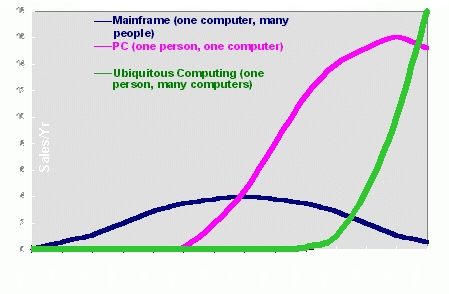
\includegraphics[width=10cm]{images/majortrends.png}
	\caption{Tri vala u računarstvu (preuzeto u edukacijske svrhe, ne valja slika)}
	\label{fig:majortrends}
\end{figure}

\section{Zahtjevi}
Analiziranjem zahtjeva na sveprisutno i prožimajuće računarstvo, može se
zaključiti nešto:
\begin{itemize}
  \item Mali uređaji
  \item Umrežavanje
  \item Sakupljanje podataka i razmjena u okruženju bez prisustva korisnika
  \item Otvoreno računarstvo radi podložnosti promjene softwarea i uređaja
  (Java ili CLR ili nekaj takvo -> bytecode)
\end{itemize}

Još jedna lista zahtjeva na sveprisutno
\begin{itemize}
  \item Uređaj za prikaz, terminal, korisnički interface
  \item Ekonomična cijena
  \item Širok mrežni opseg
  \item Sistem nevidljivih datoteka (bez znanja o direktorijima, nazivu
  datoteka, lokaciji td.)
  \item Automatska instalacija - migracija s jednog računala na drugi
  \item Personaliziranost informacija
  \item Privatnost (ima puno personaliziranih informacija, što ako se netko
  dokopa?)
\end{itemize}

koje su glavne potrebe za rad sa sveprisutnim sustavima (mala energija,
procesna moć, interakcija s okolinom)

\section{Primjena}

Udri brigu na veselje u ovom poglavlju natuć za sva vremena xD

Pametni gradovi, pametni prostori, internet stvari.

Aspekt integracije: postojeće stvari -> nova tehnologija (orjentacija u muzeju
s mobitelom)

Primjene u urbanom računarstvo:
\begin{itemize}
  \item Javne i komercijalne infrastrukture
  \item Mobilne i druge bežične mreže
  \item Kolektivni transport
  \item Plaćanje
  \item Sigurnost i nadgledanje
  \item Rasprostranjeno reklamiranje
  \item Pametna arhitektura
  \item Spektakularni urbani događaji
  \item Mobilni tehnološki uređaji
  \item Osobna komunikacija
  \item Servisi socijalnih mreža
  \item Urbana umjetnost?
\end{itemize}

Urbani krajolik -> skriveni slojevi mogu postati vidljivi, svojevrsni izum
mikroskopa.

Urbano računarstvo -> ljudi koji žive u urbanoj stredini mogu imati mnogo
različitih interesa ali imaju jednu stvar koja im je zajednička: mjesto gdje
žive (ovo bi se moglo primjeniti na činjenicu da svi imaju isti cilj u šopingu)

\chapter{Preporučiteljski sustavi}
\section{Uvod u preporučiteljske sustave}
Preporučiteljski sustavi su, ukratko rečeno, skup programskih alata i tehnika
koji iz relativno velikog i nepreglednog skupa karakteriziranih informacija
krajnjem korisniku, koji je opet na neki način karakteriziran, filtriraju
informacije o mogućim preferencijama tog korisnika. Općenito, možemo reći da je
jednostavan model preporučiteljskog sustava dan formulom:
\begin{equation}
\label{eq:elementarniModel}
	R \leftarrow U \times I
\end{equation}
gdje je $R$ rezultat, tj. predikcija \engl{prediction, recommendation},
preferencije korisnika $U$ \engl{ user} koji je zatražio preporuku, tj.
filtriranje sadržaja , a $I$ predmet nad kojim se vrši predikcija preferencije
\engl{item}. Traženje potencijalnih preporuka za korisnika $U$ tada se u
najjednostavnijem slučaju svodi na kombiniranje profila njegovih preferencija s
profilima predmeta u skupu svih predmeta dostupnih algoritmu za filtriranje.
Dakle, preporuka $R$ zapravo je predviđanje ocjene korisnika $U$ za
traženi predmet $I$. Krajnji rezultat na kraju jest najčešće lista od $n$
najboljih preporuka, tj. pretpostavki da bi korisnik te predmete ocjenio
najbolje \engl{top -- $N$ list}. 

Gornji model ima dva osnovna i lako uočljiva ograničenja:
\begin{enumerate}
  \item Traženje preporuka za korisnika svodi se na iscrpno pretraživanje
  prostora predmeta dostupnih algoritmu za filtriranje
  \item Rezultat je preporuka kojoj fali bilo kakav kontekst.
\end{enumerate}

Da bismo doskočili ovim problemima, razmotrit ćemo razne modele preporuke od
kojih su neke već dobro poznati i korišteni algoritmi. Za početak, uvedimo u
formulu \ref{eq:elementarniModel} općeniti kontekst preporuke:
\begin{equation}
\label{eq:elementarniModelSKontekstom}
	R \leftarrow U \times I \times C
\end{equation}
gjde je $C$ kontekst u kojem korisnik $U$ traži preporuku.

Predmet se shvaća generički i on može varirati ovisno o kontekstu primjene,
primjerice, artikli u internet trgovini, knjige u digitalnim knjižnicama, pjesme
i filmovi namultimedijalnim servisima, rezultati pretraživanja na tražilicama,
osobe na društvenim mrežama, smjerovi kretanja u prostoru i u ovisnosti s
vremenom itd. Svaki predmet u korišten od strane algoritma za filtriranje obično
je opisan nekim karakteristikama koji variraju u ovisnosti o kontekstu predmeta.
Tako primjerice neka pjesma može biti opisana žanrom, trajanjem i izvođačem, a
knjiga isto tako žanrom, autorom i brojem stranica. Unositi težine za pojedine
ocjene karakteristika predmeta nije uobičajeno jer na taj način dolazi do
subjektiviziranja rezultata filtriranja na manji skup osoba, ali s druge strane
gledano, nije ni nemoguće.

S druge strane, korisnici sustava imaju različite scenarije korištenja
preporučitelja od kojih su osnovni filtriranje neželjenog sadržaja iz velikih
baza podatak i savjetovanje pri nedostatku vlastite kompetencije za izbor
sadržaja (referenca: ono čudo koje te pita kaj te interesira). Korisnici imaju
svoje preferencije koje su u ovom slučaju uglavnom opisane težinama jer prema
različitim potrebama određene karakteristike predmeta nad kojima se vrši
filtriranje mogu biti zanimljivije, odnosno manje zanimljive.

Interakcijom korisnika sa sustavom omogućuje se praćenje njegovih odabira,
treniranje preporučitelja te kroz analizu profila korisnika i njegovih osobnih
preferencija stvaranje modela za preporuku predmeta na nekoliko načina. Podaci
koje korisnik ostavlja u sustavu u osnovi se mogu podijeliti u dva skupa:
\begin{enumerate}
  \item Implicitni
  \item Eksplicitni
\end{enumerate}
Implicitni podaci su oni podaci koje je sustav prikupio od korisnika bez da ga
je to eksplicitno zatražio. Takvi podaci mogu biti primjerice, demogravski
podaci, točnije, šire područje iz kojeg korisnik koristi sustav a jednostavno se
doznaje iz baze podataka dodijeljenih područja \engl{scope} IP adresa.
Također, pod implicitne podatke spadaju i akcije korisnika u sustavu koje se
mogu doznati iz sjedničkih zapisa, kao i tzv. klikovi na određene poveznice
unutar sustava.

S druge strane, eksplicitni podaci su oni koje korisnik ostavlja s namjerom,
primjerice koristeći ankete o svojim preferencijama, ostavljajući povratnu
informaciju na ponuđene predmete \engl{feedback} ili odgovarajući na bilo
koji način na upite o pojedinim predmetima.

U općem slučaju, preporučiteljske sustave razlikujemo prema načinu filtriranja i
analiziranja informacija, a razlikujemo četiri osnovna načina (tj. jedan način
pseudofiltriranja i tri načina filtriranja):
\begin{enumerate}
  \item Filtriranje neovisno o korisniku \engl{Non -- personalized
  filtering}
  \item Filtriranje zasnovano na sadržaju \engl{Content -- based
  filtering}
  \item Filtriranje zasnovano na suradnji \engl{Collaborative
  filtering}
  \item Hibridne tehnike filtriranja odnosno preporučivanja
\end{enumerate}

Povijesno gledano, razvoj preporučiteljskih sustava započeo je devedesetih
godina prošlog stoljeća, a nemalo je populariziran $2006$. g. svojevrsnim
natjecanjem \glqq The Netflix Prize \grqq kada je poznati pružatelj multimedije
na zahtjev ponudio nagradu od \$$1,000,000$ američkih dolara za tim koji razvije
preporučitelj bolji od taga postojećeg sustava \glqq Cinematch \grqq za određeni
postotak.
Ovo je ostavilo velik utjecaj na razvoj preporučitelja prvenstveno zbog
činjenice da je u uvjetima natjecanja navedeno da rezultati i principi rada
razvijenih preporučitelja moraju biti javno objavljeni i dostupni
%referenca

\section{Filtriranje neovisno o korisniku}
%TODO negdje ubaciti kako zapravo dobiti preporuku (top N)
Osnovni model filtriranja jest filtriranje neovisno o korisniku. Model preporuke
koji proizlazi iz ovakvog načina filtriranja, strogo gledano, ne može biti
preporučitelj jer preporuka ne ovisi strogo o korisniku. Drugim riječima, svaki
korisnik koji zatraži preporuku od ove vrste filtriranja dobit će istu
preporuku. Ovu tvrdnju mogli bi jednostavnije prikazati relacijom:
\begin{equation}
\label{eq:filtriranjeNeovisnoOKorisniku}
	R \leftarrow I
\end{equation}
gdje je $R$ predikcija, tj. preporuka, a $I$ predmet. Iz relacije
\ref{eq:filtriranjeNeovisnoOKorisniku} očigledno je da je predikcija funkcija
isključivo predmeta, pa kao takva ne može biti smatrana punokrvnim
preporučiteljem.

Razmjerno jednostavna predožba ovog modela jest rejting \engl{Rating}.
Uzmimo za primjer neki servis za ocjenjivanje i korisničke recenzije
ugostiteljskih objekata. Neka svaki korisnik koji je koristnio uslugu nekog od
objekata ima pristup sustavu u kojem može u više kategorija ostaviti ocjenu iz
nekog intervala s prisanom recenzijom. Također, neka svaki korisnik ima
mogućnost ocijeniti uslugu brojčanom ocjenom iz intervala od jedan do pet. Model
preporučitelja u tom slučaju bio bi opisan s:
\begin{equation}
\label{eq:skupOcjena}
	S = \{1, 2, 3, 4, 5\}
\end{equation}
\begin{equation}
\label{eq:prosjek}
	R = \lfloor \frac{\sum_{i=1}^{N} s_i}{N} \ast 10 \rfloor
\end{equation}
gdje je $S$ skup mogućih ocjena, $R$ konačan rejting predmeta, $N$ ukupan broj
korisnika koji su ocjenili taj predmet, a $s_i$ ocjena $i$-tog korisnika. Iako,
izgrađeni model preporuke strogo gledano nije preporučitelj, on to ipak čini
posredno nudeći korisniku ono što su drugi korisnici obilježili kao poželjnije.
Ovakav model obično koriste usluge s povratnom informacijom korisnika
\engl{ Feedback}, npr. \emph{eBay}, \emph{Tripadvisor} i \emph{Zagat}.
Elemente ovog preporučitelja prikazane relacijama \ref{eq:skupOcjena} i
\ref{eq:prosjek} možemo varirati kako bi prilagodili izgrađeni model drugim
sustavima, primjerice:
\begin{itemize}
  \item Skup ocjena $S$. Ovisno o potrebi, moguće je skup proširiti do potrebnog
  broja ocjena, imajući na umu da veća granulacija nije nužno bolja, kao i da
  može biti beskorisna u vidu onemogućenja korisnika da predmet ocjeni spontano,
  a da neće biti vidljiva u krajnjem rezultatu. Također, granulaciju je moguće
  povećati dozvoljavanjem ocjena van skupa cijelih brojeva.
  \item Prikaz rezultata $R$. U formuli \ref{eq:prosjek} prije zaokruživanja
  prosjek je pomnožen faktorom $10$ radi eliminacije decimala. Moguće je
  odabrati neki drugi prikaz rezultata, primjerice u postotcima.
\end{itemize}
Sam način ocjenjivanja ne mora nužno biti eksplicitna dodjela ocjene. Moguće je
primjerice koristiti sustav glasovanja \engl{Vote up/down} \engl{Vote
up/down}.
Najpoznatiji primjeri koji koriste takve ocjene su \emph{Reddit} i \emph{StackOverflow}.

U općem slučaju modeli preporučitelja zasnovani na ovakvoj vrsti filtriranja
imaju dvije mane:
\begin{itemize}
  \item Zavaravanje korisnika od strane rejtinga koji je, neovisno o načinu
  prikaza, i dalje samo prosjek pojedinačnih ocjena.
  \item Nedostatak konteksta za preporuke.
\end{itemize}

Nedostatak konteksta za preporuke posebno se manifestira prilikom asocijativnog
preporučivanja. Uzmimo za primjer da tražimo preporuku za neki predmet koji je
dodatak na neki već postojeći predmet, primjerice, tražimo preporuku za preljev
za sladoled.
%TODO a gdje ovo utrpati
Izgradimo sada jednostavan model prema kojem bi mogli dobiti nepersonaliziranu
preporuku za predmet koji ovisi o drugom predmetu. Neka su $X$ i $Y$ skupovi
svih korisnika koji su kupili proizvode $X$ i $Y$ respektivno.

Intuitivno se nameće da ukoliko je više korisnika kupilo proizvod $X$ i uz njega
proizvod $Y$ da će i ostalim korisnicima (koji traže preporuku) proizvod $Y$
odgovarati uz proizvod $X$. Elementarnom algebrom skupova možemo dakle
zaključiti da se predikcija za nekog korisnika može izraziti relacijom:
\begin{equation}
\label{eq:naivnaNepersonaliziraniTemp}
	R = \frac{\mid X \cap Y \mid}{\mid X \mid}
\end{equation}
Osnovni problem proizlazi iz činjenice da su određeni predmeti neovisno
popularni. Primjerice, u nekom dućanu, moguće je da većina korisnika kupuje neki
predmet pa može doći do lažne korelacije popularnog predmeta s nekim drugim
predmetom. Drugi problem je nepostojanost veze između predmeta iz skupa $X$ i
$Y$ u smislu asocijativnosti. Ukoliko je $X$ skup sladoleda, a $Y$ skup
preljeva, korisniku bi kao preporuku trebalo izdvojiti preljeve za sladoled iz
skupa $Y$. 

\begin{equation}
\label{eq:nepersonalizirani}
	R = \frac
		{\frac
			{\mid X \cap Y \mid}
			{\mid X \mid}}
		{\frac
			{\mid \overline{X} \cap Y\mid}
			{\mid \overline{X} \mid}}
\end{equation}

Preporuka korisniku na kraju se jednostavno svodi na prikaz prvih $N$ najboljih
prosječnih ocjena.

Naivni preporučitelj preporuku može dati korištenjem intuitivno izvedive
formule:
\begin{equation}
\label{eq:naivnaNepersonalizirani}
	R = \frac{X \cap Y}{X}
\end{equation}
gdje su $X$ i $Y$ skupovi svih korisnika koji su kupili proizvode 

\section{Filtriranje ovisno o korisniku}
Za razliku od filtriranja neovisnog o korisniku, filtriranje ovisno o korisniku
uzima u obzir korisnika i njegove preferencije.
\subsection{Filtriranje zasnovano na sadržaju}
Razmotrimo situaciju kada ne tretiramo korisnike ili predmete kao osnovne
(atomarne) jedinice, nego ih možemo opisati nekim kategorijama, primjerice,
demografskim podacima za korisnika, autorom i izdavačem ako je predmet neka
knjiga i sl. Preporučivanje zasnovano na sadržaju u osnovi dovoi u vezu
prikupljene preferencije korisnika, bilo eksplicitno, bilo implicitno. Neka je u
sustavu koji koristi preporučitelj zasnovan na sadržaju svaki predmet opisan
tekstualnim medapodacima i vektorom:
\begin{equation}
\label{eq:vektorKarakteristika}
	\boldsymbol{X_i} = 
		\big[ 
			\boldsymbol{w_{1,i}}, 
			\boldsymbol{w_{2,i}}, 
			\boldsymbol{w_{3,i}}, 
			\ldots, 
			\boldsymbol{w_{N,i}} 
		\big]^T
\end{equation}
gdje je $\boldsymbol{w_{j,i}}$ kvantitativni, tj. brojčani opis neke $j$-te
karakteristike za $i$-ti predmet. Težina je neka proizvoljno odabrana metrika
koja može varirati od jednostavnog broja pojavljivanja, uključujući $0$/$1$
pristup (karakteristika je primjenjiva, odnosno karakteristika nije
primjenjiva) do precijznijih metrika. Sličnost između dva predmeta moguće je
tada izraziti kosinusom kuta između vektora njihovih karakteristika. 
\begin{equation}
\label{eq:kosinus}
	\boldsymbol{cos}(\boldsymbol{V}_1, \boldsymbol{V}_2) = 
		\frac
			{\boldsymbol{V}_1 \ast \boldsymbol{V}_2}
			{\|\boldsymbol{V}_1\| \times \|\boldsymbol{V}_2\|}
\end{equation}
Tu još negdje ubaci da svaka karakteristika može imati svoju težinu, u smislu da
neka karakteristika može biti važnija.
Također, neka za svakog korisnika postoji korisnički profil sa dostupnim
preferencijama korisnika dostupnim u vektorskom zapisu gdje $i$-ta komponenta
vektora predstavlja težinu te karakteristike za korisnika. Tada je na sličan
način moguće izraziti kompatibilnost promatranog korisnika i predmeta. U
ovisnosti o kontekstu primjene, vektore je poželjno i normalizirati.
Jedna od većih prednosti ovog načina filtriranja je što može stvarati preporuke
neovisno o tome je li za predmet davana povratna informacija ili ne. Drugim
riječima, ovaj način filtriranja iznimno je prikladan na početku rada sustava
jer nema problema s takozvanim hladnim početkom \engl{ Cold start}. Isto
tako, prikladan je za primjene gdje je moguće relativno dobro strukturiranim
karakteristikama opisati predmete. S druge strane, nepogodan je ukoliko ga
se implementira u sustave gdje korisnici dolaze rijetko ili relativno često
mijenjaju preferencije. Zbog svega navedenog, ova vrsta filtriranja uglavnom se
upotrebljava u sustavima za pregledavanje vijesti, personaliziranim servisima za
multimediju, video na zahtjev i sl.

Nešto tu ne štima vezano uz težine. Komponente vektora zapravo su kvantitativni
opis, brojka, to nisu težine. Težine, koje predstavljaju koja je karakteristika
korisniku koliko važna su u drugom vektoru?

\subsection{Filtriranje zasnovano na suradnji}
Suradnički pristup dijametralno je suprotan sadržajnom pristupu. Princip rada
ove vrste filtriranja suradnja je između pojedinih korisnika odnosno predmeta.
Definicija ove vrste suradnje zapravo leži u određivanju sličnosti između dvaju
korisnika ili predmeta, a glavna premisa jest da preferencije predmeta uglavnom
važe za sve korisnike koji imaju iste interese ili su slično ocijenili slične
predmete. Primjerice, razmatranjem slučaja gdje dva različita korisnika dodijele
dvije relativno slične ocjene nekom predmetu, zaključak jest da je vjerojatnost
da su ta dva korisnika slično ocjenila i neke druge predmete razmjerno velika. S
druge strane, veća je vjerojatnost da će neki korisnik ocjeniti slično neka dva
predmeta ako su ih i ostali korisnici slično ocjenili.

Zbog usporedbi i rada na dvije različite razine, korisničkoj i predmetnoj, ovaj
preporučitelj se u osnovi dijeli na dvije moguće tehnike:
\begin{itemize}
  \item Korisnik-korisnik \engl{User-user, Neighbourhood-based,
  Memory-based}
  \item Predmet-predmet \engl{Item-item, Item-based, Model-based}
\end{itemize}

\subsubsection{Korisnik -- Korisnik}
Suradničko filtriranje na relaciji između korisnika koji traži preporuku i
ostalih korisnika sustava svodi se na predikciju ocjene korisnika koji traži
preporuku za neki predmet na osnovu ocjena njemu bliskih ljudi gdje je bliskost
dva korisnika dobro definirana nekom metrikom, npr. Pearsonovim koeficjentom
korelacije (\ref{eq:pearsonKorisnik})

\begin{equation}
\label{eq:pearsonKorisnik}
	R = \frac
			{\sum_{i \epsilon I} 
				\big[
					(r_{k,i} - \overline{r_k}) \ast
					(r_{u,i} - \overline{r_u})
				\big]
			}
			{
				\sqrt{{\sum_{i \epsilon I} (r_{k,i} - \overline{r_k})^2}} \ast 
				\sqrt{{\sum_{i \epsilon I} (r_{u,i} - \overline{r_u})^2}}
			}
\end{equation}

gdje je $w_{q,u}$ težina između aktivnog korisnika $k$ i korisnika $u$, $i$ skup
predmeta koje su ocijenila oba korisnika, $r_{u,i}$ ocjena koju je korisnik $u$
dodijelio predmetu $i$, a $\overline{r_u}$ srednja vrijednost svih ocjena koje
je dodijelio korisnik $u$.

Alternativno, ocjene korisnika možemo predstaviti kao vektore u
$m$ - dimenzionalnom prostoru pa se težina može izraziti preko skalarnog
produkta kao kosinus kuta između ta dva vektora:

\begin{equation}
\label{eq:pearsonKosinus}
	w_{k,u} = 
		\cos{(\vec{r_k}, \vec{r_u})} = 
		\frac
			{\vec{r_k} \ast \vec{r_u}}
			{\|\vec{r_k}\| \times \|\vec{r_u}\|} = 
		\frac
			{\sum_{i=1}^m r_{k,i} \ast r_{u,i}}
			{\sqrt{\sum_{i=1}^m r_{k,i}^2} \ast \sqrt{\sum_{i=1}^m r_{u,i}^2}}
\end{equation}

Mana pristupa \ref{eq:pearsonKosinus} jest nedostatak negativnih ocjena.

Neka je $K$ skup svih korisnika nekog sustava. Također, neka je $k$ korisnik iz
skupa $K$ koji traži preporuku za neki predmet. Tada je susjedstvo $N$
korisnika $k$ definirano kao
\begin{equation}
\label{eq:susjedstvo}
	N = K \backslash \{k\}
\end{equation}

S obzirom na relaciju \ref{eq:susjedstvo} i metriku za ocjenu bliskosti
(\ref{eq:pearsonKorisnik}) ili \ref{eq:pearsonKosinus} dan je algoritam za
filtriranje na relaciji više korisnika:
\ref{algo:korisnik-korisnik}
\begin{algorithm}
	\caption{Korisnik-korisnik filtriranje}
	\label{algo:korisnik-korisnik}
	\begin{algorithmic}
		\STATE{\textbf{Ulaz:} $k$ - korisnik za kojeg se traži predikcija. $N$ -
		susjedstvo korisnika}
		\STATE{\textbf{Izlaz:} Predikcija $p$ ocjene korisnika $K$ za predmet $P$.}
		\STATE{topN := $20$}
		\STATE{n := length($N$)}
		\STATE{w := initVector()}
		\FOR{($i := 0; i < n; inc(i)$)}
			\STATE{$w_i := calculatePearson(k, N_i)$}
		\ENDFOR
		\STATE{sort(w)}
		\STATE{$suma := 0; tezine := 0$}
		\FOR{($i := 0; i < topN; inc(i)$)}
			\STATE{$suma := suma + w_i * N_i$}
			\STATE{$tezine := tezine + w_i$}
		\ENDFOR
		\STATE{$p := suma / tezine$}
		\RETURN{p}
	\end{algorithmic}
\end{algorithm}

Algoritam se ugrubo svodi na:
\begin{enumerate}
  \item Dodjelu težine svim susjedima korisnika $k$.
  \item Odabir $n$ susjeda koji imaju najveće težine s obzirom na korisnika $k$
  gdje je broj tih susjeda ($topN$) određen empirijski.
  \item Izračun predviđanja ocjene korisnika $k$ iz težinskog prosjeka ocjena
  odabranih korisnika
\end{enumerate}

Ovaj pristup je relativno efikasan i jednostavan za implementaciju, ali druge
strane, računalno postaje vrlo zahtjevan ako se primjeni na velike baze podataka
korisnika i predmeta. U algoritmu \ref{algo:korisnik-korisnik} se može vidjeti
da $for$ petlja ima $N$ prolazaka, a za svaki taj prolazak računa se Pearsonov
koeficjent korelacije dan formulom \ref{eq:pearsonKorisnik} ($I$ puta).
Složenost tada iznosi:
\begin{equation}
\label{eq:slozenostKorisnik}
	O(N \ast I)
\end{equation}

Iako ocjene \ref{eq:slozenostKorisnik} pokazuje je ovisnost linearna,
ipak se vidi da povećanjem broja korisnika ili predmeta dolazi do
značajnog povećanja potrebnog broja operacija za izračun preporuke. 
Valja dodati i da je algoritam \ref{algo:korisnik-korisnik} pojednostavljena
verzija algoitma, pa ni ocjena \ref{eq:slozenostKorisnik} ne može biti uzeta
kao konačna.

\subsubsection{Predmet -- Predmet}
S obzirom na nedostatke prethodne tehnike u performansama, inženjeri poznate
internetske trgovine \emph{Amazon.com} predložili su sličan pristup ali iz druge
perspektive gdje se ne traže sličnosti između korisnika, nego između predmeta
\cite{amazon}. Kao i kod prethodno opisanog pristupa i algoritma
\ref{algo:korisnik-korisnik}, metrika za ocjenu sličnosti između predmeta je
Pearsonov koeficjent korelacije, u ovom slučaju definiran kao:

\begin{equation}
\label{eq:pearsonPredmet}
	R = \frac
			{\sum_{u \epsilon U} 
				\big[
					(r_{u,i} - \overline{r_i}) \ast
					(r_{u,j} - \overline{r_j})
				\big]
			}
			{
				\sqrt{{\sum_{u \epsilon U} (r_{u,i} - \overline{r_i})^2}} \ast 
				\sqrt{{\sum_{u \epsilon U} (r_{u,j} - \overline{r_j})^2}}
			}
\end{equation}

gdje je $U$ skup svih korisnika koji su ocjenili predmete $i$ i $j$, $r_{u,i}$
ocjena korisnika $u$ za predmet $i$, a $\overline{r_i}$ srednja ocjena $i$-tog
predmeta za sve korisnike. Predviđanje ocjene korisnika $k$ za predmet $i$
računa se korištenjem težinskog prosjeka:
\begin{equation}
\label{eq:tezinskiProsjek}
	p_{k,i} = 
		\frac
			{\sum_{j \epsilon N} r_{k,j} \ast w_{i,j}}
			{\sum_{j \epsilon N} \|w_{i,j}\|}
\end{equation}
gdje je $N$ susjedstvo predmeta ocjenjenih od strane korisnika $k$ najsličnijih
predmetu $i$. Jedan od najpoznatijih preporučitelja na svijetu, internetska
trgovina \emph{Amazon.com} koristi patentirani hibridni algoritam baziran na
ovoj tehnici.
\section{Hibridni tehnike}
\begin{enumerate}
  \item Težinski - ocjena predmeta preporuke računa se iz svih dostupnih
  preporučiteljskih tehnika u sustavu. Najjednostavniji primjer jest linearna
  kombinacija preporuka. Neki sustavi koji koriste ovu tehniku kombiniraju
  preporuke zasnovane na suradnji i preporuke zasnovane na sadržaju uz
  kalibraciju težina u ovisnosti o povratnoj informaciji korisnika.
  \item Izmjenični - kod ove tehnike sustav koristi neki predefinirani kriterij
  za izmjenu tehnike preporuke, primjerice, neka je dan sustav koji inicijalno
  za svakog korisnika koristi preporuku zasnovanu na suradnji. Ako sustav tom
  tehnikom ne može stvoriti preporuku određenog nivoa pouzdanosti, rpebacuje se
  na preporuku zasnovanu na sadržaju.
  \item Miješani - ova tehnika računa preporuke iz više elementarnih
  preporučitelja i prikazuje ih simultano.
  \item Kombinacija obilježja - jedan od načina za spajanje suradnjičkog i
  sadržajnog preporučitelja jest interpretirati informacije suradničkog
  preporučitelja kao dodatne podatke koji čine ulaz sadržajnog preporučitelja.
  \item Kaskada - ova tehnika predstavlja svojevrsnu dvorazinsku preporuku. Prvo
  jedan preporučitelj relativno grubo rangira potencijalne kandidate, a nakon
  toga drugi preporučitelj radi precizniju razdiobu. Tehnika je posebno pogodna
  za one slučajeve kada jedan preporučitelj ne može dovoljno precizno generirati
  predviđanja za preporuke predmeta.
  \item Pojačavanje obilježja - tehnika kod koje je generirano predviđanje ili
  klasifikacija predmeta jednog preporučitelja pripojena slijedećoj
  preporučiteljskoj tehnici u nizu.
  \item Meta razina - izlaz jednog preporučitelja je ulaz drugog preporučitelja.
\end{enumerate}

Konkretne primjene preporučiteljskih sustava u heterogenim okolinama, danas se
svode u velikoj mjeri na različite hibride osnovnih tehnika. Velike industrije
trgovine i zabavnih sadržaja u praksi imaju autorska algoritamska rješenja
hibridnih preporučitelja.
\section{Moguća područja primjene}
\section{Preporučiteljski sustavi u sveprisutnom računarstvu}
Primjena preporučiteljskih sustava u sveprisutnom računarstvu logična je
posljedica ne samo činjenice da je sveprisutno računarstvo računarstvo kao takvo
pa u njemu postoji interes za preporukom, nego i činjenice da se u njemu
generiraju velike količine podataka pa se preporučiteljski algoritmi mogu
primjeniti kao filtri podataka. O podacima sveprisutnom računarstvu praktički
je nemoguće govoriti bez konteksta u kojem se nalaze. Taj kontekst može se
definirati kao bilo koja informacija o okolnostima, predmetima ili uvjetima
koje okružuju korisnika, a smatra se relevantnom za interakciju između
korisnika i sveprisutnog računalnog okruženja \cite{RanganathanCampbell}.

Tri najvažnija aspekta kontekseta su \cite{schilit1994context}:
\begin{enumerate}
  \item Gdje se korisnik sustava nalazi
  \item U društvu kojih je drugih korisnika sustava
  \item Koji resursi se nalaze u blizini
\end{enumerate}

Koje su specifičnosti? Nisam ni sam ziher, algoritam vjerojatno mora biti
prilagođen filtiranju ogromne količine nestrukturiranih podataka, kontekst
vremena i prostora je najbitniji, predmeti preporuke su iz puno više različitih
domena nego npr na amazonu, pa ih je teže opisati.

Primjer preporučiteljskog sustava koji se djelomično nalazi u sveprisutnom
računarstvu jest algoritam koji koristi \emph{Foursquare}. \emph{Foursquare} je
servis koji preporučuje lokale na temelju preferencija korisnika, njegovih
ocjena sličnih lokacija te ocjena njegovih najbližih prijatelja i stručnjaka
koje prati \cite{FoursquareAbout}. Kod ovog preporučitelja vidljiv je prostorni
kontekst u smislu preporučivanja

specifičnosti, koji postoje, mobilni uređaji, foursquare itd.
%-------------------------------------------------------------------------------
%  CHAPTER: Izgrađeni model preporučiteljskog sustava
%-------------------------------------------------------------------------------
\chapter{Izgrađeni model preporučiteljskog sustava}


\section{Preporučiteljski sustavi s izraženom prostornom i vremenskom
komponentom}

Priča o postojećim preporučiteljima i kako nemaju prostorno vremenskih
komponenti 

Osnovni problem s kojim se konvencionalni preporučiteljski sustavi susreću (a
time i popularniji radni okviri i biblioteke koji ih implementiraju) jest
izostanak bilo kakve potpore za prostorne i vremenske komponente koje
su se pokazale neophodne za rad sa sveprisutnim sustavima.
%Za sveprisutno prostor i vrijeme su jedne od bitnijih stavki (referenca?)

\section{Naš model}
Znači cijeli model treba opisati, od ocjenjivanja do apsolutno svega

\begin{equation}
\label{eq:DefModel}
	R \leftarrow U \times I \times C
\end{equation}

\begin{equation}
\label{eq:Context}
	C \leftarrow T \times S
\end{equation}

Izražen prostorno vremenski kontekst (općenito)
dvije razine reinforcementa. preporučitelj neće raditi online, tj. akcije iz
trenutnog sessiona ne utječu na preporuke u tom istom sessionu. tek kad se
session commita (po izlasku iz sustava) profili se zbrajaju i preporuke postaju
aktualne koje je pravo vrijeme za reinforcement dva profila -> privremeni i
trajni profil pa zbroj nakon kupnje netko svaka dva tjedna kupuje jabuke pa mu
se svaka dva tjedna kupuju jabuke (recurring)


Tu bi u principu trebalo ubaciti the algoritam
* fade out efekt
akcije(u konzumu)
I kolaboracija i sadržaj
- kod sadržaja, gdje je udaljenost manja od nekog broja (i fizička udaljenost)
- račun udaljenosti je apstrahiran

Možda sekcija kontekst pa onda napisati nešto generički o kontekstu pa onda
podsekcije prostor i vrijeme
Sekcija za svaku komponentu, korisnika i predmete, fino opisati od čega se
sastoje itd.

Kakve su ocjene, koje su skale

\section{Prostorna komponenta}

S obzirom na kompleksnost postupka modeliranja prostora, prostorna komponenta
konteksta modelirat će se poednostavljeno, i to kvadratnom mrežom
(slika \ref{fig:StoreGrid}). Iako se na prvi pogled tako čini, to nije
ograničenje jer modeliranje prostora u kojem će korisnici tražiti preporuku
najčešće nije slobodno, tj. korisnik se u takvim prostorima kreće putem koji mu
je dostupan. Primjer je dućan u kojem se korisnik može kretati između polica, a
očito je i razumno da se ne može kretati \emph{preko} polica.
%TODO: ružno napisano, refactor
Dostupne puteve za korisnika može se čuvati u npr. riječnicima
\engl{Dictionary}, tj. parovima $kljuc \rightarrow vrijednost$ gdje je $kljuc$
neko polje kvadratne mreže a $vrijednost$ lista svih \emph{susjednih} polja do
kojih je moguće doći iz polja $kljuc$. Minorna mana ovog pristupa jest
dvostruko spremanje putova jer ako se iz polja $p_1$ može doći u polje $p_2$,
onda se iz polja $p_2$ može doći u polje $p_1$. Dvostruko spremanje može se
izbjeći nauštrb vremenu pretraživanja dvostrukih putanja, a za relativno malu
memorijsku uštedu, čak i kod modeliranja vrlo velikih prostora.
%TODO: Manhattan distance
%TODO: refactor text
Ako se kvadratnu mrežu i dostupne putove kretanja prikaže kao neusmjereni
težinski graf, onda se taj prostor može predstaviti \emph{matricom
susjedstva}, a kako je takva matrica simetrična, spremati se može samo npr.
gornja trokutasta matrica, čime se postiže svojevrsna rijetka popunjenost
matrice \engl{Sparse Matrix}.
%TODO: i ovo refactor
%treba napisati kako su različite namjene dijkstre i A* itd.
Prednost predstavljanja mreže i prostora grafom jest i postojanje nebrojeno
mnogo pouzdanih i efikasnih algoritama za traženje najkraćeg puta između dva
vrha, odnosno dva polja. Neki od njih su npr. \emph{Dijkstrin algoritam},
\emph{Bellman-Ford algoriam} ili \emph{A$\ast$ algoritam}.

\begin{figure}[htb]
	\centering
	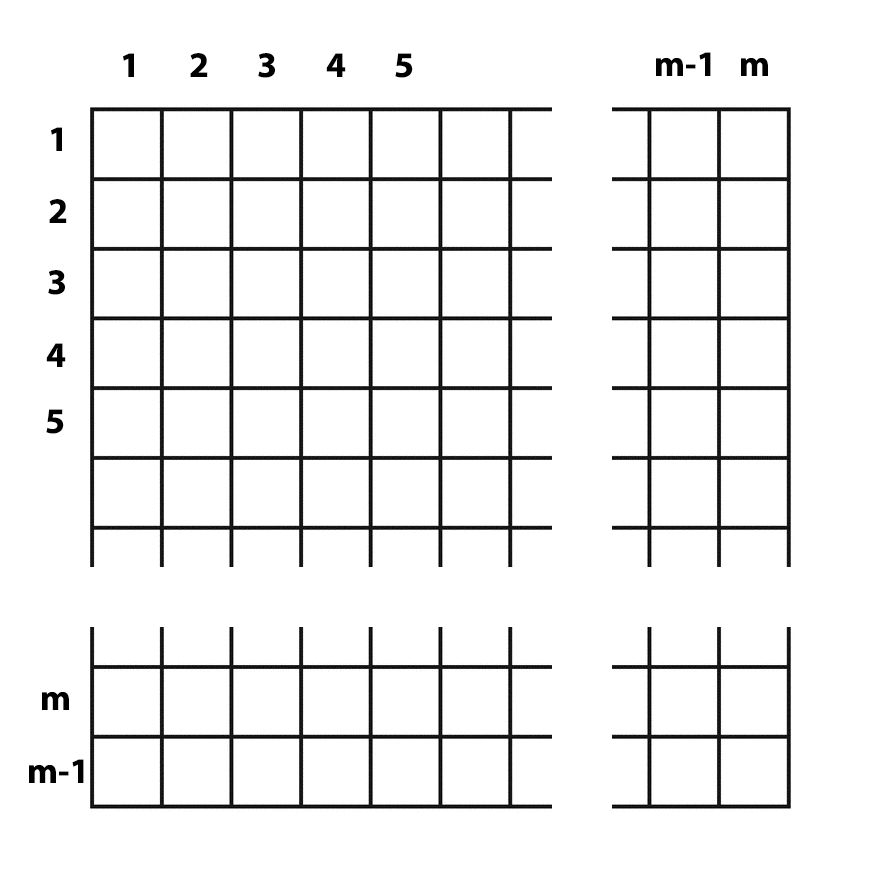
\includegraphics[width=7cm]{images/grid.png}
	\caption{Tlocrt prostora modeliran kvadratnom mrežom}
	\label{fig:StoreGrid}
\end{figure}

\section{Vremenska komponenta}

Vremenska komponenta koja se uzima u obzir u modelu preporučitelja također je
zapravo komponenta konteksta u kojem se nalazi korisnik. 

uuuu, korisnik može za određeni proizvod imati funkciju koja opisuje kakve on
ima vremenske preferencije s obzirom na taj proizvod. ili funkcija može
opisivati samo one trenutke kada se stavlja korisnik u situaciju da traži
preporuk

Jedna takva funkcija može biti primjerice tzv. \emph{Gaussova krivulja}
(slika \ref{fig:Gauss1}). Ona je pogodna zbog činjenice da prosječan korisnik
prosječnu akciju u kojoj će tražiti preporuku u principu traži u jednom kraćem
vremenskom intervalu. Drugim riječima, pojedini predmeti preporuke za nekog
korisnika u vremenski svjesnom preporučiteljskom sustavu bit će zanimljivi samo
jedan kraći interval.
\begin{equation}
	\label{eq:BellFunc}
	f(x;a,b,c) = \frac
	{
		1
	}
	{
		1 + \mid\frac{x - c}{a}\mid^{2b}
	}
\end{equation}
gdje je $x$ varijabla, a $a$, $b$ i $c$ parametri kojima se regulira oblik
krivulje:
\begin{itemize}
  \item $a$ - širina vrha
  \item $b$ - nagib porasta i pada, oblik vrha
  \item $c$ - pomak na $x$ osi
\end{itemize}

\begin{figure}[htb]
	\centering
	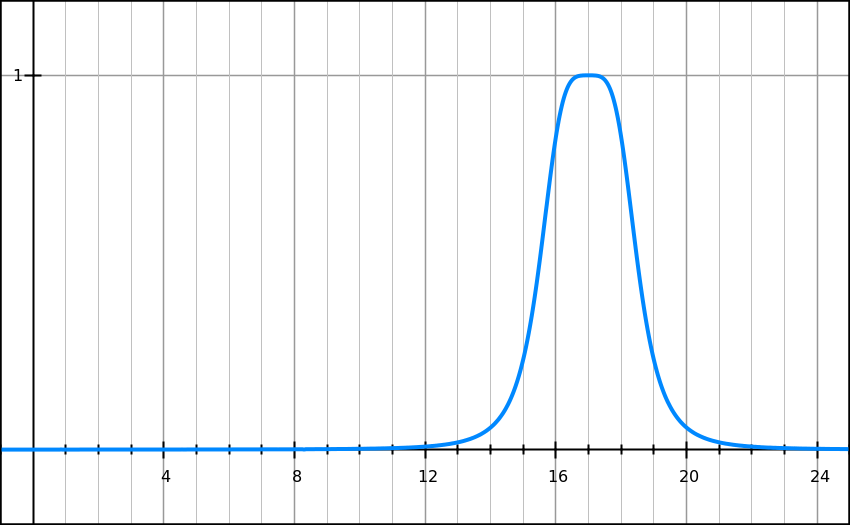
\includegraphics[width=12cm]{images/zvonolika1.png}
	\caption{Preferencija korisnika za predmet na dnevnoj skali}
	\label{fig:Gauss1}
\end{figure}

S druge strane, skala ne mora biti dnevna, može biti i tjedna te se funkciju
može zadati po dijelovima (puno kompleksnije situacije). % Tu mi fali neka slika 
% funkcije pod više dijelova i na tjednoj skali
Znači, funkcija može biti na više različitih skala i može odražavati
preferenciju za predmet ili preferenciju za traženje preporuke općenito

\begin{figure}[htb]
	\centering
	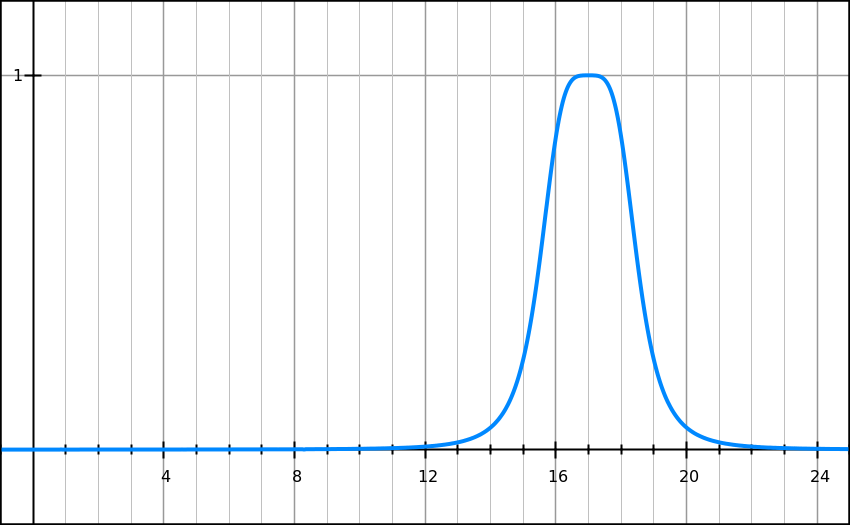
\includegraphics[width=12cm]{images/zvonolika1.png}
	\caption{Preferencija korisnika za predmet na dnevnoj skali}
	\label{fig:Gauss2}
\end{figure}

S obzirom na matematičku analizu koja stoji iza računa za pronalazak funkcije,
one se mogu zadati i diskretno, npr. kroz vektor uzoraka funkcije. Ta diskretnu
funkciju može se koristiti kao takva ili se može procesom interpolacije naći
njezin eksplicitni zapis. Pogodne metode interpolacije mogu npr. biti
interpolacija polinomom višeg stupnja ili interpolacija splajnovima
\engl{Spline}.

u funkcija može biti kontinuirana, a može biti i uzorkovana i
pohranjena u nekom polju. y os funkcije tada je vrijednost koju korisnik
pridaje nekom proizvodu u neko doba dana. ne mora biti ni doba dana, može biti
doba tjedna. diskretizirane funkcije mogu se interpolirati polinomima višeg
stupnja ili splajnovima

%TODO: refactor
Vremenska komponenta omogućava i praćenje obrazaca ponašanja korisnika, pa time
i predviđanje ponavljanja ponašanja \engl{Recurring}.

Vremenska komponenta podrazumjeva i tzv. \emph{efekt blijeđenja} \engl{Fade-out
effect}. Ako korisnik kod kojeg je uočen neki obrazac akcija prestane provoditi
tu akciju, preporučitelj će prestati primati pobudu za održavanje te akcije.
Međutim, neće je odmah zanemariti nego će se vremenska komponenta, tj. funkcija
koja opisuje tu komponentu, lagano gušiti nekom drugom funkcijom, primjerice
recipročnom eksponencijalnom funkcijom:

\begin{equation}
	\label{eq:RecipExp}
	g(x) = e^{-x}
\end{equation}

Tada će ukupan rezultat vremenske komponente konteksta biti:

\begin{equation}
	\label{eq:Gusenje}
	T \leftarrow f(x) \ast g(x)
\end{equation}

gdje je $f(x)$ funkcija koja opisuje vremensku komponentu konteksta nekog
korisnika za neki predmet, a $g(x)$ funkcija koja guši tu komponentu.
primjer. Ovdje također postoji mogućnost da se funkcija $g(x)$ zada diskretno,
tj. po uzorcima.

akcije

\section{Modeliranje korisnika}
multiplus profil

\begin{enumerate}
  \item multiplus profil, znamo tko što voli, tj. imamo profil korisnika
  \item dopuna profila? kroz šetnju, kroz zadržavanje, kada kupi?
  \item cold start profil?
\end{enumerate}

Profil:
\begin{enumerate}
  \item Proizvodi, skupine proizvoda, redovi? -> stablo?
  \item vektor preferencija
\end{enumerate}

%Novi chapter%
\chapter{Ispitivanje modela}
\section{Ispitni scenarij}
Osmišljavanje ispitnog scenarija pokazalo se natprosječno zahtjevnim radi
pokušaja da takav scenarij obuhvati i ispita sve segmente kontekstualno svjesnog
preporučitelja. S druge strane, takav scenarij je morao biti realno
ostvariv, u smislu da ne bude sintetički osmišljen nego da u realnom
svijetu postoji takva situacija u kojoj će se osmišljeni preporučiteljski
model moći implementirati i koristiti. Na kraju je odabrana prosječna
svakodnevna aktivnost većine potencijalnih korisnika ovakvog sustava, a to je
odlazak u kupovinu.

%TODO: gdje se nalaze podaci o policama?
Ispitni scenarij podrazumjeva generički srednje velik dućan u kojem se
može naći mješovita roba, dakle, i prehrana i neprehrana. Radi jednostavnosti, a
bez značajnijeg utjecaja na krajnji ishod, tlocrt dućana modeliran je mrežastom
strukturom prikazanom na slici \ref{fig:StoreGrid}. U dućanu se na svakom mjestu
mogu nalaziti radio oznake \engl{beacon} kojima mogu biti obilježeni:
\begin{itemize}
  \item Neka lokacija u dućanu, npr. red polica
  \item Skupina proizvoda
  \item Konkretan proizvod
\end{itemize}
Ovdje se nameće pitanje je li potrebno radio oznakama obilježiti sve
potencijalne predmete preporuke. Sa strane sustava, podrazumjeva se
posjedovanje točnih lokacija svake radio oznake, a poznavanjem točnih lokacija
te poznavanjem rasporeda u dućanu, interpolacijom možemo aproksimirati lokaciju
korisnika u trenutcima kada je on između radio oznaka. Svakoj radio oznaci
pridodani su i neki metapodaci od kojih je najvažniji jedinstveni identifikator
u sustavu.

%TODO: beacon opis
Svaka radio oznaka ima određeni domet signala kojim razašilje \engl{broadcast}
svoj jedinstveni identifikator. Kada se mobilni uređaj nađe u dometu signala, on
prima taj jedinstveni identifikator te može utvrditi \emph{RSS} \engl{Received
signal strength}. 

\begin{figure}[htb]
	\centering
	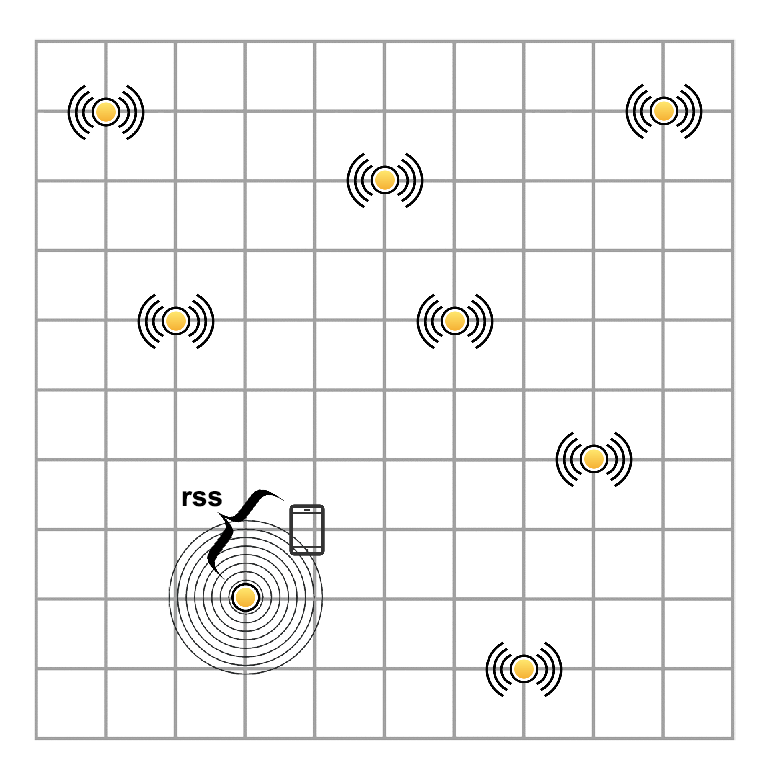
\includegraphics[width=9cm]{images/gridbeacons1cell.png}
	\caption{Grafički prikaz radio oznake i mobilnog telefona}
	\label{fig:RssOneCell}
\end{figure}

Slika \ref{fig:RssOneCell} prikazuje slučaj kada je mobilni
uređaj u dometu jedne radio oznake. U tom slučaju može se smatrati da je
korisnik zainteresiran za ono što radio oznaka obilježava. S druge strane,
ako se korisnik nađe u dometu dva ili više radio oznaka (slika
\ref{fig:RssTwoCells}), onda se jednostavno uzima signal one radio oznake čiji
je \emph{RSS} u tom trenutku jači. Naime, \emph{RSS} opada s udaljenošću pa se s
pravom može smatrati da jači \emph{RSS} nužno povlači veću fizičku blizinu
korisnika u odnosu na pripadajuću radio oznaku, tj. ono što ta radio oznaka
obilježava.

\begin{figure}[htb]
	\centering
	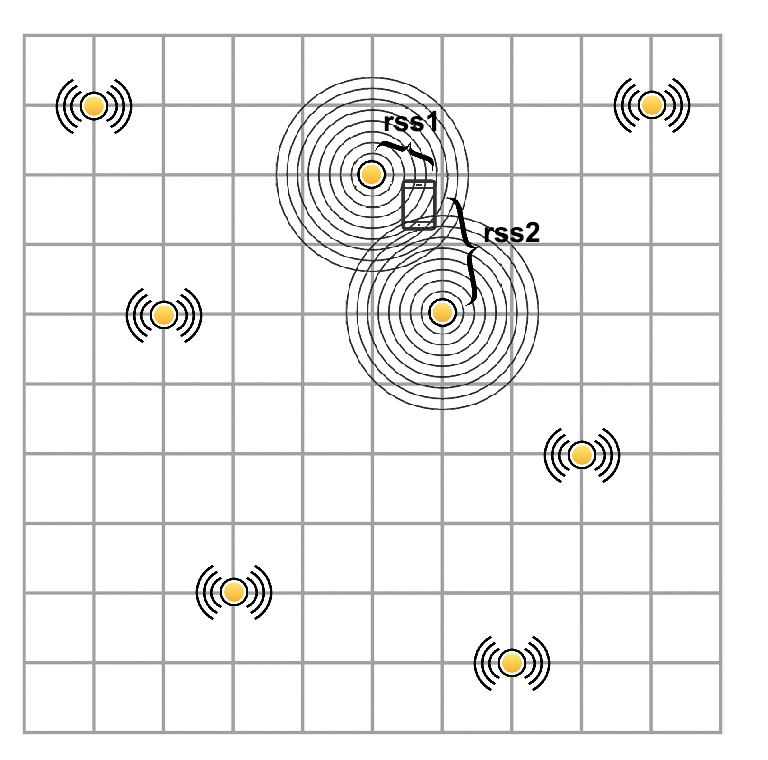
\includegraphics[width=9cm]{images/gridbeacons2cells.png}
	\caption{Grafički prikaz višestrukog prijama signala s radio oznaka}
	\label{fig:RssTwoCells}
\end{figure}

Također, uzima se u obzir i vrijeme zadržavanja korisnika u blizini radio
oznake. Ukoliko je korisnik proveo manje vremena od neke empirijski određene
vremenske granice $t_min$, onda se može smatrati da korisnik nije iskazao
interes za predmet koji radio oznaka obilježava.
U obzir valja uzeti i orjentaciju korisnika. Nerijetko je moguće da korisnik
bude u dometu signala radio oznake, a fizički nije usmjeren prema predmetu koji
ona označava. Korištenjem magnetometra na pametnom uređaju i poznavanjem
razmještaja radio oznaka u prostoru, može se jednostavno utvrditi je li korisnik
iskazao interes za obilježeni predmet ili je okrenut od njega.
%zadržavanje -> reinforcement prvog stupnja

Izvor podataka je dobro enkapsuliran pa se može reći da mora implementirati
sučelje s određenom opremom, a ta oprema je:
\begin{itemize}
  \item Komunikacijski radio, npr. \emph{WLAN} \engl{Wireless LAN} -- koristi
  se za svu komunikaciju sa poslužiteljima po pitanju dohvaćanja metapodataka o
  radio oznakama, traženje preporuke itd.
  \item Magnetometar -- koristi se utvrđivanje je li korisnik okrenut prema
  radio oznaci ili od nje. % 
  \item Akcelerometar -- koristi se za utvrđivanje gibanja korisnika. Ako je
  korisnik u pokretu, zanemaruju se podaci sa ulaza za očitavanje radio oznaka
  \item Bluetooth -- koristi se za komunikaciju s radio oznakama
\end{itemize}

Takav izvor u praksi može biti bilo koji moderniji mobilni telefon ili tablet.

\section{Simulacija primjene}
%TODO: treba negdje ubaciti kako se stvar može generalizirati
Opis načina testiranja
Opisati inpute i outpute, konfiguraciju itd.

Ulazi i izlazi
\begin{enumerate}
  \item logovi (id + rss)
  \item multiplus id
  \item lokacija beacona s id-em
  \item multiplus profil (kontekstualizirani), vremenski
  \item tendencija kretanja
\end{enumerate}
\begin{enumerate}
  \item lista s obzirom na lokaciju i vrijeme
  \item s obzirom na očekivani profil kupnje
\end{enumerate}

timestamp -> popis beacona + rss
magnetometar i akcelerometar
shadow preporuke (može u globalni model) -> implicitna preporuka u kojoj korisnika
preko akcija vodimo do onoga što njemu treba
beacon id -> proizvod i lokaciju

out -> za trenutnu lokaciju -> u kojem smijeru dalje i koji proizvodi idući (topN)

\section{Provođenje testiranja}
Opis testnog scenarija u smislu kako smo polijepili beacone po feru, hodali,
zaustavljali se itd.
\section{Rezultati testiranja}
Prikazati rezultate, jelte

\chapter{Zaključak}
Zaključak.

\bibliography{literatura}
\bibliographystyle{fer}

\begin{sazetak}
Sažetak na hrvatskom jeziku.

\kljucnerijeci{Ključne riječi, odvojene zarezima.}
\end{sazetak}

\engtitle{Recommender systems in ubiquituous computing}
\begin{abstract}
Abstract.

\keywords{Keywords.}
\end{abstract}

\end{document}
